\chapter{Introdução}\label{ch:introducao}
A mecânica dos fluidos é uma área muito complexa da engenharia, mesmo com todo o avanço tecnológico e computacional 
nem sempre é possível projetar com precisão sem se valer de uma análise prévia da ação de esforços sobre algum material.
O estudo da ação do ar sobre estruturas pode ser um fator determinante entre o sucesso e o fracasso de um projeto.

A análise aerodinâmica, se bem conduzida, pode apresentar dados confiáveis ao projetista para o apoio na tomada 
de decisão. Uma das maneiras de realizar estes estudos é através das leis de similaridade para replicar resultados em escalas reais. 
Assim, de uma forma menos onerosa é possível fazer esse estudo em escala reduzida e com condições controladas 
em laboratório. Os túneis de vento são as bancadas de testes para estudos de escoamento de ar, onde é possível simular cenários e avaliar a interação do fluido e estrutura.

Complementar a um controle de escoamento no túnel de vento estão os instrumentos para as grandezas físicas 
(pressão e velocidade). O tubo de Pitot e a Sonda de anemômetro de fio quente são exemplos de instrumentos 
de medição, usados dentro desses canais aerodinâmicos.

A operação desses equipamentos dentro do túnel de vento pode ser de forma manual ou automatizada. A primeira tende a 
gerar imprecisões, como o posicionamento incorreto do sensor em relação ao seus eixos vertical e horizontal, além de 
um gasto considerável de tempo e energia, pois o operador, para fazer o reposicionamento do equipamento, deve desligar 
o túnel, abri-lo e posicionar o equipamento para fazer a próxima medição, gerando assim incertezas de operação. Já a 
atuação automatizada resolve todos os problemas acima citados, porém o processo de implantação é mais dispendioso. 
A Figura \ref{fig:sisantigozoom} apresenta de forma esquemática a seção de teste do túnel de vento com 
seu equipamento atual de medição.

\begin{figure}[H]
\centering
\caption{Suporte atual da mesa.}\label{fig:sisantigozoom}
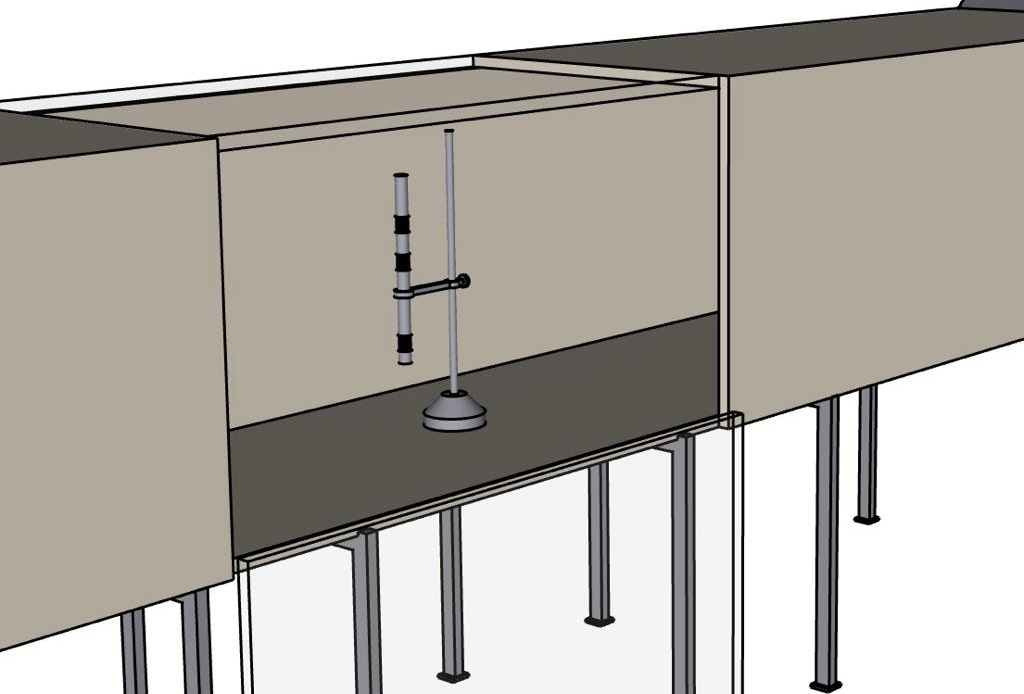
\includegraphics[scale = 0.33]{figuras/sisantigozoom}
\end{figure}

A realização desse trabalho justifica-se por desenvolver um equipamento que agrega um sistema de coordenadas 
bidimensional para posicionamento de instrumentos de medição no túnel de vento do Laboratório de Sistemas Térmicos  
da Universidade Federal do Rio Grande.

\section{Objetivo Geral}\label{sec:objetivogeral}

Projetar um dispositivo para o posicionamento automático de equipamentos de medições dentro de um túnel de vento, 
para facilitar o processo de caracterização do escoamento de forma automatizada.

\section{Objetivos Específicos}\label{sec:objetivoesp}

	\begin{itemize}
		\item Projetar a mesa cartesiana.
		\item Criar o sistema eletrônico de comunicação entre a mesa e o software.
		\item Desenvolver o software que comandará a mesa cartesiana.
	\end{itemize}

\section{Estrutura do trabalho}\label{sec:estruturatrab}

Na primeira seção são apresentados: o tema do projeto, os objetivos, 
a justificativa e a estrutura do trabalho.

A segunda seção apresenta a revisão bibliográfica, a fim de ser referência neste estudo e para fundamentar 
a base teórica utilizada no trabalho.

A terceira seção apresenta a metodologia e detalhamento dos componentes do projeto em si, 
que envolve o projeto do sistema mecânico, sistema eletrônico, desenvolvimento do software 
e a integração dos sistemas.

A quarta seção apresenta os resultados e discussão.

A quinta seção apresenta as considerações finais, críticas e sugestões para trabalhos futuros.

Por último são dispostas as referências bibliográficas e apêndices.